The Open Data Lab is in the business of hosting data sets with various levels of openness. We encourage all users to make their data as open as practicable. Currently there is a purchased data set reffered to as 'Healthy Markets' in the ODL (it contains financial information). And we are bringing a Numismatic data set online. There are also various data sets for student research  projects hosted on the open data lab.

At the end of 2018-2019 academic year the total amount of data in the lab was  13.6\,TB. This is predominantly from the Healthy Markets Dataset. Figure~\ref{fig:s3cost} shows the data usage overtime.

\begin{figure}[!hbtp]
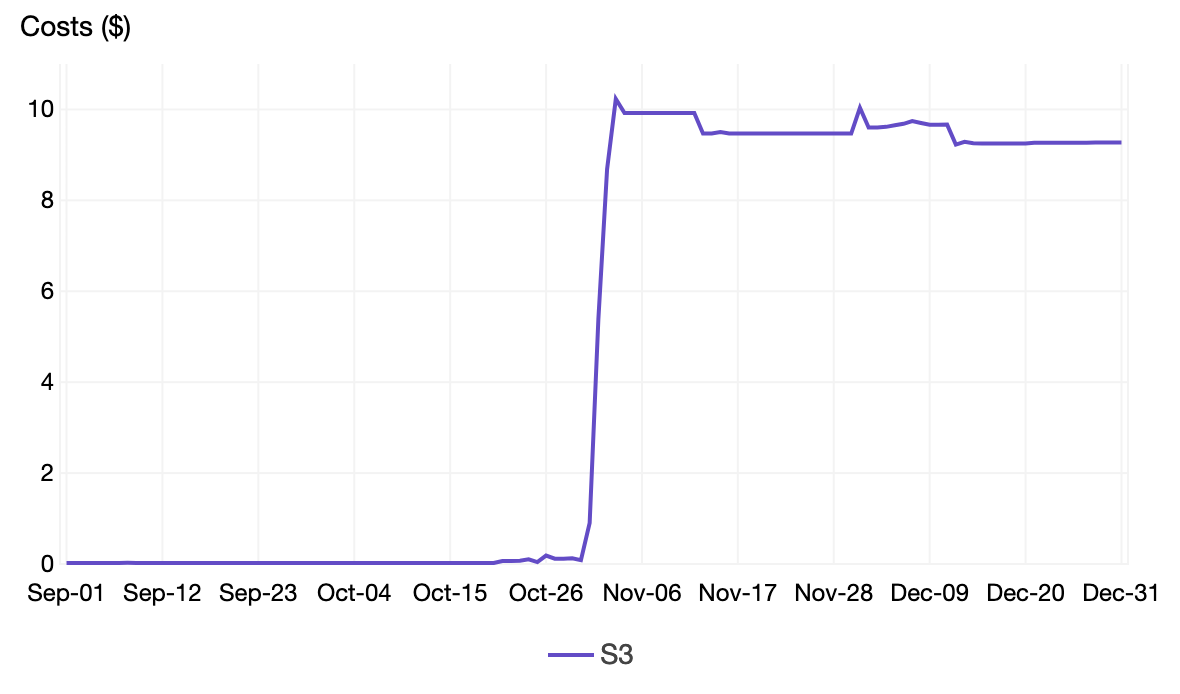
\includegraphics[width=0.85\textwidth]{images/odl-s3-usage-2018.png}
\caption{Healthy Markets daily cost for S3 service (2018)}
\label{fig:s3cost}
\end{figure}



\section{Healthy Markets}
The Healthy Markets dataset was purchased by the University under liscense for use by  all members of the university. The Open Data Lab is responsible for storage and providing access to the dataset. Narjessadat Seyeditabari (Narges Tabari) is responsible for facilitating research on the dataset and is the primary user of the dataset.

The data set is 13\,TB and is stored in an S3 bucket named 'odl-hmtt'. This bucket is private to users of the Open Data Lab and is accessed through a SageMaker instance. To copy the data from it's source at Healthy Markets we used the AWS CLI and it took several days with a total cost of \$1 for REST actions and \$17 for the EC2 instance to manage the transfer. The current cost to store the data set is \$290 per month. These costs are covered by the Healthy Markets PTAO.

Section~\ref{sec:hmt} contains the report on research activities with this data set.

\section{Numismatic}
Dr. Ethan Gruber from the American Numismatic Society is in possession of a Linked Data Set  and wants to make it open with the Open Data Lab. He is interested in establishing a SPARQL endpoint for the  dataset. An S3 bucket (odl-nept) has been provisioned to store the data for the project and we will be making the data set open in 2020.